\documentclass[journal]{IEEEtran}
\usepackage{amsmath,amssymb,amsthm}
\usepackage{graphicx}
\usepackage{booktabs}
\usepackage{cite}
\usepackage{xcolor}
\usepackage{algorithm}
\usepackage{algpseudocode}
\usepackage{tikz}
\usetikzlibrary{positioning,arrows.meta,fit,shapes.geometric,calc}
\usepackage[hidelinks]{hyperref}

\newtheorem{proposition}{Proposition}
\newtheorem{corollary}{Corollary}
\newcommand{\todo}[1]{\textcolor{red}{[TODO: #1]}}
\newcommand{\vect}[1]{\mathbf{#1}}
\newcommand{\E}{\mathbb{E}}
\DeclareMathOperator{\tr}{tr}
\DeclareMathOperator{\diag}{diag}
\graphicspath{{figures/}}

\begin{document}

\title{Digital-Twin-Aided Fronthaul Compression of\\ Channel Information for Cell-Free Open RAN}
\author{[Authors]%
\thanks{Draft generated on 9 October 2026 from the experiment index in \texttt{paper1/experiments.md}. Red text marks items that are still open.}}

\maketitle

\begin{abstract}
Centralized precoding in cell-free Open RAN (O-RAN) requires every O-RU to forward the channel information (CI) it estimates from sounding reference signals (SRS) to the O-DU, a load that reaches several Gbit/s per O-RU for wideband massive arrays. We show that if the O-DU and the O-RUs share a ray-traced digital twin of the site, i.e., a geometric channel knowledge map, together with a posterior on each UE position, most of this CI need not cross the fronthaul. Both ends synthesize twin channels over the position-uncertainty region, derive the same per-link Karhunen--Lo\`eve basis, and allocate bits across links, UEs and dimensions by reverse water-filling of the twin eigenvalues on a first-order sum-rate model, without any signaling. The O-RU sends block-floating-point coefficients with a measured scale and a noise-matched width, and spends the remaining bits on an angle--delay residual layer for components the twin misses. We show that the high-resolution rate redundancy of such shared-prior coding splits exactly into a basis-mismatch term and an allocation-mismatch term whose sum is bounded by a Kullback--Leibler divergence, and that the spectral-efficiency loss of centralized regularized zero forcing is governed by the leakage of compression errors into the other UEs' beams, which the twin predicts. In a Sionna RT urban site with four O-RUs, the scheme reaches 95\% of the uncompressed sum spectral efficiency with 1.9, 4.9 and 7.7~kbit per O-RU and SRS occasion for 8, 16 and 32 UEs, i.e., 13\% to 3\% of what exact distributed Gram-matrix precoding needs on the uplink alone. It degrades gracefully under geometric, material and scattering mismatch, and a closed loop in which the O-DU localizes the UEs on the twin removes the need for external positioning.
\end{abstract}

\begin{IEEEkeywords}
Cell-free massive MIMO, Open RAN, fronthaul compression, digital twin, channel knowledge map, source coding, centralized precoding.
\end{IEEEkeywords}

\section{Introduction}

Cell-free massive MIMO lets many distributed access points serve the UEs jointly~\cite{ngo2017cellfree,interdonato2019ubiquitous}. Its best spectral efficiency (SE) is obtained with centralized processing, where a central unit holds the channels of all UEs to all access points and computes a network-wide MMSE or regularized zero-forcing (RZF) precoder~\cite{bjornson2020making}. In an Open RAN (O-RAN) deployment with the 7.2x split~\cite{polese2023oran}, the access points are O-RUs and the central unit is an O-DU. The O-RU is the natural place to estimate the uplink SRS channels, and the O-RAN fronthaul specification already defines how an O-RU conveys SRS channel information (CI) to the O-DU, with block floating point (BFP) and beamspace compression~\cite{oran_cus_v22}. The cost is large: with 64 antennas, 273 PRBs, 32 UEs with four SRS ports each, an SRS every ten slots and BFP9, the CI of one O-RU is about 4.2~Gbit/s, roughly 16\% of its downlink user-plane payload. This is the fronthaul bottleneck of centralized cell-free precoding that we address.

Existing remedies either change where the processing happens or compress generic representations. Distributed processing exchanges low-dimensional statistics instead of channels; for RZF, each O-RU can send its local Gram matrix and the O-DU returns the inverse, which reproduces centralized RZF exactly~\cite{li2017decentralized}, but the exchange grows as $K^2$ per PRB group in both directions and requires a round trip and local computation at every O-RU. Team precoding handles unequal channel knowledge at the transmitters~\cite{miretti2022team}. Fronthaul compression for cloud RAN has been studied in depth for baseband signals, exploiting correlation with side information at the decoder~\cite{park2013joint,park2014fronthaul}, and recent work jointly designs quantized precoders and bit allocation~\cite{demir2026jointquant}, adapts compression to channel statistics~\cite{li2025adaptive}, or reduces the dimension of uplink signals under fronthaul constraints~\cite{kim2026fronthaul}; O-RAN compression schemes have been compared for distributed MIMO~\cite{rahmani2025oran,lagen2021modcomp}. These works compress signals or precoders with generic or statistically learned transforms; none exploits a deterministic model of the propagation environment that both ends of the fronthaul hold.

Site-specific digital twins built by ray tracing~\cite{hoydis2023sionnart,alkhateeb2023dt} and channel knowledge maps (CKM)~\cite{zeng2024ckm} are becoming available, and several works use them for channel state information. A twin can generate training data for deep-learning CSI feedback~\cite{luo2025dtfeedback,luo2026calibration}; zone-specific subspaces predicted by a twin can reduce pilot overhead in channel estimation~\cite{alikhani2025zone}; an environment basis stored per grid cell supports CSI prediction from few pilots~\cite{cai2025ecb}; radio maps enable reduced-pilot CSI tracking~\cite{zheng2025radiomap}; and the sensitivity of twin-aided estimation to site geometry and calibration has been quantified~\cite{delmoro2026geometry}. In 3GPP, site-specific (``localized'') AI models improve two-sided CSI compression over global models~\cite{3gpp38843}. All of these use the twin as a prior or as a training set for estimation or feedback at a single base station. Three questions remain open for the fronthaul of a cell-free O-RAN: how to turn a twin shared by the O-DU and the O-RUs into a source code with essentially no side information on the link; what rate such a code needs when the twin is wrong and the UE position is uncertain; and how to distribute bits over many O-RUs when the end goal is the SE of a centralized precoder rather than the reconstruction error of each link.

\textbf{Contributions.}
\begin{itemize}
\item \emph{Shared-twin source coding.} Both ends sample the position posterior of each UE with a shared seed, synthesize twin channels over the resulting region, and compute the same per-link Karhunen--Lo\`eve transform (KLT). Bit widths per link and dimension follow from reverse water-filling of the twin eigenvalues on a first-order sum-SE model and need no signaling. The O-RU quantizes with a measured block scale and noise-matched widths, and an angle--delay residual layer covers what the twin misses (Section~\ref{sec:method}).
\item \emph{Rate analysis.} We show that the high-resolution redundancy of shared-prior transform coding equals a basis-mismatch term plus an allocation-mismatch term, both nonnegative and jointly bounded by the Kullback--Leibler divergence between the true and the twin covariance. We also characterize how the effective dimension of the region subspace grows with the position uncertainty, the array aperture and the bandwidth (Section~\ref{sec:rate}).
\item \emph{Leakage law.} Under centralized RZF the SE loss due to CI compression is almost entirely leakage into other UEs' beams. A first-order SINR model with a leakage factor $\gamma$ captures it; $\gamma$ falls with the number of UEs and is predicted by the twin alone (Section~\ref{sec:leakage}).
\item \emph{Closed loop without external positioning.} The O-DU reuses the region samples as particles, localizes each UE on the twin from the reconstructed CI, and returns the posterior to the O-RUs with about 32~bit per UE (Section~\ref{sec:loc}).
\item \emph{Evaluation.} In a Sionna RT urban site with four O-RUs and realities that depart from the twin in geometry, materials, vehicles and diffuse scattering, we compare against angle--delay (beamspace-type) compression, a point twin, grid-cell environment bases~\cite{cai2025ecb}, site-wide KLT and twin-trained autoencoders, and exact distributed Gram RZF (Section~\ref{sec:results}).
\end{itemize}

\textbf{Notation.} Bold lowercase and uppercase letters denote vectors and matrices; $(\cdot)^{H}$ is the conjugate transpose; $\mathcal{CN}(\vect{0},\vect{R})$ is the circularly symmetric complex Gaussian distribution; $\|\cdot\|$ is the Euclidean norm; $\binom{N}{n}$ is the binomial coefficient.

\section{System Model}\label{sec:model}

\begin{figure}[t]
\centering
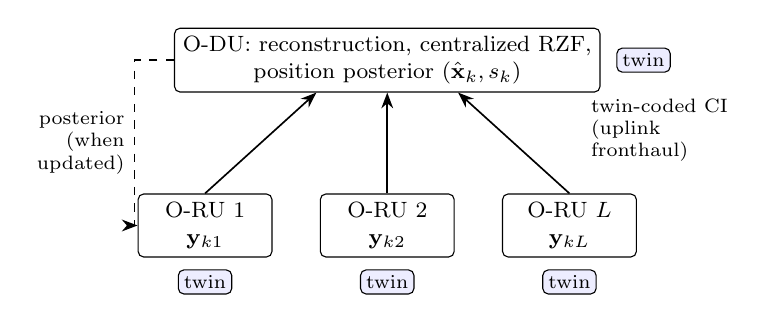
\begin{tikzpicture}[font=\footnotesize,
  box/.style={draw, rounded corners=2pt, align=center, minimum height=8mm, inner sep=3pt},
  twin/.style={draw, rounded corners=2pt, fill=blue!7, font=\scriptsize, inner sep=2pt},
  arr/.style={-{Stealth[length=2mm]}, semithick}]
\node[box, minimum width=34mm] (du) {O-DU: reconstruction, centralized RZF,\\ position posterior $(\hat{\vect{x}}_k,s_k)$};
\node[twin, right=2mm of du] (tdu) {twin};
\node[box, minimum width=17mm] (r2) at ($(du)+(0,-21mm)$) {O-RU 2\\ $\vect{y}_{k2}$};
\node[box, minimum width=17mm, left=6mm of r2] (r1) {O-RU 1\\ $\vect{y}_{k1}$};
\node[box, minimum width=17mm, right=6mm of r2] (rL) {O-RU $L$\\ $\vect{y}_{kL}$};
\foreach \r in {r1,r2,rL} {\node[twin, below=1.5mm of \r] {twin};}
\foreach \r/\x in {r1/-9mm,r2/0mm,rL/9mm} {\draw[arr] (\r.north) -- ([xshift=\x]du.south);}
\node[font=\scriptsize, align=left, anchor=west] at ($(rL.north)+(1.5mm,8mm)$) {twin-coded CI\\ (uplink\\ fronthaul)};
\draw[arr, dashed] (du.west) -- ++(-5mm,0) |- node[pos=.25, left, font=\scriptsize, align=right] {posterior\\ (when\\ updated)} (r1.west);
\end{tikzpicture}
\caption{Cell-free O-RAN with a shared twin. Each O-RU sends twin-coded SRS channel information on the fronthaul; the O-DU reconstructs it, precodes, and returns the position posterior used by both ends to build the code.}
\label{fig:system}
\end{figure}

\subsection{Network and SRS Channel Information}
We consider a cell-free O-RAN with $L$ O-RUs, each with $M$ antennas, serving $K$ single-antenna UEs over $F$ PRB groups in TDD (Fig.~\ref{fig:system}). The channel between UE $k$ and O-RU $l$ is stacked over antennas and PRB groups into $\vect{h}_{kl}\in\mathbb{C}^{N}$, $N=MF$. In each SRS occasion O-RU $l$ obtains the noisy CI
\begin{equation}
\vect{y}_{kl}=\vect{h}_{kl}+\vect{n}_{kl},\qquad \vect{n}_{kl}\sim\mathcal{CN}(\vect{0},\nu\vect{I}_N),
\end{equation}
where channels are normalized so that the UE thermal noise per resource element is one and $\nu$ is the estimation-noise variance. O-RU $l$ may spend at most $B_l$ bits per SRS occasion on the CI of all its links. The O-DU reconstructs $\hat{\vect{h}}_{kl}$, forms $\hat{\vect{H}}_f\in\mathbb{C}^{K\times LM}$ for each PRB group, and computes the centralized RZF precoder
\begin{equation}\label{eq:rzf}
\vect{W}_f=\hat{\vect{H}}_f^{H}\big(\hat{\vect{H}}_f\hat{\vect{H}}_f^{H}+K\vect{I}_K\big)^{-1},
\end{equation}
with columns scaled to power $1/K$. The SE of UE $k$ is $\mathrm{SE}_k=\frac{1}{F}\sum_f\log_2(1+\mathrm{SINR}_{k,f})$, evaluated with the true channels. Our figure of merit is the sum SE as a fraction of the sum SE obtained with the uncompressed noisy CI, as a function of the fronthaul bits per O-RU and SRS occasion.

\subsection{Digital Twin and Position Knowledge}
The O-DU and all O-RUs hold the same digital twin of the site. In practice this is a geometric CKM~\cite{zeng2024ckm}: for each grid point and O-RU, a list of propagation paths with complex gains per antenna, delays and departure angles, computed offline by ray tracing. From it either end can synthesize the twin CFR $\vect{g}_{kl}(\vect{x})$ of a UE at position $\vect{x}$. The real channel $\vect{h}_{kl}$ differs from $\vect{g}_{kl}$ at the true position because of unmodeled scatterers, geometry and material errors, and diffuse scattering. Both ends also share a Gaussian posterior $\mathcal{N}(\hat{\vect{x}}_k,s_k^2\vect{I}_2)$ on each UE position, with $s_k^2=\sigma_k^2+s_0^2$, where $\sigma_k$ is the position error and $s_0=1$~m is a tolerance for twin geometry errors. Section~\ref{sec:loc} shows how the O-DU obtains the posterior itself.

\subsection{Reference Schemes and Accounting}
All schemes are billed for every bit they send on the O-RU-to-O-DU link: coefficient mantissas, block exponents, width fields, counts and indices. Coefficients are quantized with noise-matched BFP, a variant of O-RAN BFP9: blocks of 12 coefficients in send order, a 4-bit exponent, and per block the narrowest mantissa (2 to 9 bits) whose step does not exceed $\kappa\sqrt{\nu}$ with $\kappa=2$, signaled by a 3-bit width field. Sets of $n$ indices out of $N$ cost $\lceil\log_2\binom{N}{n}\rceil$ bits. The exact distributed alternative, a local Gram matrix per PRB group followed by a central inverse~\cite{li2017decentralized}, costs $K^2F$ real values per O-RU on the uplink (billed at 9~bit each) and as much again on the downlink.

\section{Shared-Twin Source Coding}\label{sec:method}

\subsection{Region Twin Subspace}
For UE $k$ both ends draw $S$ positions $\vect{x}_k^{(i)}=\hat{\vect{x}}_k+s_k\vect{u}_i$, with $\vect{u}_i\sim\mathcal{N}(\vect{0},\vect{I}_2)$ generated from a shared seed, and synthesize $\vect{g}^{(i)}_{kl}=\vect{g}_{kl}(\vect{x}^{(i)}_k)$, each referenced to the earliest arrival over all O-RUs as in downlink timing. The singular value decomposition of $\vect{G}_{kl}=[\vect{g}^{(1)}_{kl},\dots,\vect{g}^{(S)}_{kl}]$ yields the region KLT $\vect{U}_{kl}$ and the eigenvalues $\lambda_{kl,i}=\varsigma_{kl,i}^2/S$ of the twin region covariance $\hat{\vect{R}}_{kl}=\frac1S\vect{G}_{kl}\vect{G}_{kl}^{H}$, i.e., the average power of each KLT dimension over the region. We use $S=64$.

\subsection{Bit Allocation Without Signaling}
Let $E_k=\sum_{l,i}\lambda_{kl,i}$ be the predicted channel energy of UE $k$ and $D_k$ the energy of its CI error after reconstruction, summed over O-RUs, antennas and PRB groups. Section~\ref{sec:leakage} shows that the SINR of UE $k$ under centralized RZF is well described by
\begin{equation}\label{eq:proxy}
\mathrm{SINR}_k\approx\frac{a(E_k-D_k)}{1+\gamma c D_k},\quad a=\frac{N_t-K+1}{N_tFK},\quad c=\frac{K-1}{KFN_t},
\end{equation}
with $N_t=LM$ and a leakage factor $\gamma$. We take $Q_k=\log_2(1+\mathrm{SINR}_k)$ as the per-UE utility. If dimension $i$ of link $(k,l)$ receives $b$ bits per real component, its error is $\lambda_{kl,i}$ for $b=0$ and $\nu+\epsilon_b(\lambda_{kl,i}+\nu)$ otherwise, where $\epsilon_b$ is the normalized MSE of the optimal $2^b$-level uniform quantizer for a Gaussian. Both ends run the same greedy reverse water-filling: starting from $b\equiv0$, they repeatedly add one bit per real component (two bits per complex coefficient) to the dimension with the largest increase of $\sum_kQ_k$, subject to the budget $B_l$ of the O-RU that owns the link and $b\le11$, and stop when no increment increases the utility. A dimension with $\lambda_{kl,i}\le\nu$ is never sent, because quantizing its noisy coefficient leaves more error than dropping it. Since only twin quantities enter, the bit pattern needs no signaling.

\subsection{Quantization at the O-RU}
O-RU $l$ computes the coefficients $\vect{c}_{kl}=\vect{U}_{kl,\mathcal{S}}^{H}\vect{y}_{kl}$ of the allocated dimensions $\mathcal{S}$. Dimensions with the same width form blocks of 12 in eigenvalue order. Each block gets a power-of-two step from the \emph{measured} maximum magnitude (4-bit exponent), so a twin that misjudges the power of a dimension does not cause overload. If the measured maximum would need fewer bits than allocated for a step of at most $\kappa\sqrt{\nu}$, the block is sent with this narrower noise-matched width (3-bit field), and the saved bits go to the residual layer.

\subsection{Residual Layer}
The twin misses components, for example diffuse scattering. The O-RU forms the residual $\vect{r}_{kl}=\vect{y}_{kl}-\vect{U}_{kl,\mathcal{S}}\hat{\vect{c}}_{kl}$ and its angle--delay coefficients $\vect{z}_{kl}=\vect{T}^{H}\vect{r}_{kl}$, where $\vect{T}$ is the unitary two-dimensional DFT over each polarization of the planar array combined with a DFT over PRB groups. Candidates are coefficients above the universal threshold $|z_n|^2>2\nu\ln N$~\cite{donoho1994ideal}. The O-RU selects candidates of all its UEs greedily by utility gain per bit, using its own measured channel and residual energies instead of the twin prediction for its links; a coefficient costs its noise-matched BFP bits plus the marginal index cost $\log_2\frac{N-n}{n+1}$ when $n$ indices of that link are already selected. Each link carries a 10-bit count.

\subsection{Reconstruction, Signaling and Complexity}
The O-DU reconstructs $\hat{\vect{h}}_{kl}=\vect{U}_{kl,\mathcal{S}}\hat{\vect{c}}_{kl}+\vect{T}\hat{\vect{z}}_{kl}$ and applies~\eqref{eq:rzf}. Algorithm~\ref{alg:code} summarizes the procedure. Besides the billed uplink bits, the O-DU returns $(\hat{\vect{x}}_k,s_k)$ to the O-RUs, about 32 plus 8 bits per UE, only when the posterior changes. The region KLT costs $NS^2\approx3.4\times10^6$ complex multiplications per link with the snapshot method ($N=832$, $S=64$), and synthesizing $S$ CFRs from about 30 paths each costs $1.6\times10^6$. An O-RU processes only its $K$ links (about 0.7~GFLOP per update for $K=32$) and the O-DU all $KL$ links (about 3~GFLOP); bases are recomputed only when the posterior changes. A CKM storing the 32 strongest paths per O-RU on a 1-m grid over $180\times195$~m needs about 230~MB.

\begin{algorithm}[t]
\caption{Shared-twin coding of SRS CI (one SRS occasion)}\label{alg:code}
\begin{algorithmic}[1]
\Statex \textbf{Both ends} (identical, from twin and posterior only)
\For{each UE $k$}
  \State draw $\vect{x}_k^{(i)}\sim\mathcal{N}(\hat{\vect{x}}_k,s_k^2\vect{I})$, $i=1,\dots,S$ (shared seed)
  \State for each O-RU $l$: $\vect{G}_{kl}\gets[\vect{g}_{kl}(\vect{x}_k^{(i)})]_i$, $(\vect{U}_{kl},\lambda_{kl})\gets\mathrm{SVD}(\vect{G}_{kl})$
\EndFor
\State widths $b_{kl,i}\gets$ greedy reverse water-filling of $\sum_kQ_k$ in~\eqref{eq:proxy} under $\{B_l\}$
\Statex \textbf{O-RU $l$}
\State $\vect{c}_{kl}\gets\vect{U}_{kl,\mathcal{S}}^{H}\vect{y}_{kl}$; BFP with widths $b$, measured scale, noise-matched cap
\State residual $\vect{z}_{kl}\gets\vect{T}^{H}(\vect{y}_{kl}-\vect{U}_{kl,\mathcal{S}}\hat{\vect{c}}_{kl})$; keep $|z_n|^2>2\nu\ln N$
\State greedy selection over its UEs by utility gain per bit; send coefficients, indices, counts
\Statex \textbf{O-DU}
\State $\hat{\vect{h}}_{kl}\gets\vect{U}_{kl,\mathcal{S}}\hat{\vect{c}}_{kl}+\vect{T}\hat{\vect{z}}_{kl}$; RZF~\eqref{eq:rzf}; update posterior (Section~\ref{sec:loc})
\end{algorithmic}
\end{algorithm}

\section{Rate Analysis}\label{sec:rate}

\subsection{Redundancy of Shared-Prior Transform Coding}
Model the noisy CI of a link as $\vect{y}\sim\mathcal{CN}(\vect{0},\vect{C})$ with $\vect{C}=\vect{R}+\nu\vect{I}$, and let both ends use the twin prediction $\hat{\vect{C}}=\hat{\vect{U}}\diag(\hat{\vect{c}})\hat{\vect{U}}^{H}$, $\hat c_i=\lambda_i+\nu$. In the basis $\hat{\vect{U}}$ the true coefficient variances are $c_i=\hat{\vect{u}}_i^{H}\vect{C}\hat{\vect{u}}_i$; the eigenvalues of $\vect{C}$ are $\mu_i$.

\begin{proposition}\label{prop:redundancy}
Assume high resolution, all $N$ coefficients coded, and per-coefficient distortion $c_i2^{-r_i}$ at $r_i$ bits per complex coefficient. A coder that uses $\hat{\vect{U}}$ and the reverse water-filling rates $r_i=\log_2(\hat c_i/\hat\theta)$ needs, at the same total distortion, more bits than the KLT of $\vect{C}$ by
\begin{equation}\label{eq:redundancy}
\begin{aligned}
\Delta R={}&\underbrace{\log_2\frac{\det\diag(\hat{\vect{U}}^{H}\vect{C}\hat{\vect{U}})}{\det\vect{C}}}_{\text{basis mismatch}}
+\underbrace{N\log_2\frac{\mathrm{AM}(\rho)}{\mathrm{GM}(\rho)}}_{\text{allocation mismatch}},\\
&\rho_i=c_i/\hat c_i,
\end{aligned}
\end{equation}
where AM and GM are the arithmetic and geometric means. Both terms are nonnegative; the first vanishes iff $\hat{\vect{U}}$ diagonalizes $\vect{C}$, the second iff all $\rho_i$ are equal. Moreover $\Delta R\le D_{\mathrm{KL}}(\mathcal{CN}(\vect{0},\vect{C})\,\|\,\mathcal{CN}(\vect{0},\hat{\vect{C}}))/\ln2$.
\end{proposition}
\begin{proof}
See Appendix~\ref{app:proof}.
\end{proof}

Proposition~\ref{prop:redundancy} turns twin fidelity into fronthaul bits and separates two failure modes: the twin predicts the wrong directions (basis mismatch) or the wrong relative powers (allocation mismatch). A common scale error costs nothing, which motivates measuring the block scale at the O-RU. A numerical check with random 40-dimensional covariances reproduces~\eqref{eq:redundancy} exactly (17.50 bits = 15.18 + 2.32) and gives a KL bound of 26.47 bits. At low rate some dimensions are not coded and their true energy, including energy outside the twin subspace, adds directly to the distortion; this is what the residual layer addresses. \todo{split the two terms on real twin/reality pairs for each mismatch type (experiment E8).}

\subsection{Effective Dimension Under Position Uncertainty}
Write the twin CFR of a UE near $\hat{\vect{x}}$ as $\vect{g}(\vect{x})=\sum_p\alpha_p(\vect{x})\vect{a}_p(\vect{x})$, where $\vect{a}_p$ is the unit-norm space--frequency signature of path $p$ (array response at its departure angles times the delay phase ramp) and $\alpha_p$ its complex gain. Over a region with $s$ much larger than the wavelength (8.6~cm at 3.5~GHz), the phases of different paths are effectively independent across the samples, so the region covariance is close to an incoherent sum
\begin{equation}\label{eq:regioncov}
\begin{aligned}
\hat{\vect{R}}&\approx\sum_p\beta_p\,\E_{\vect{\delta}}\!\left[\vect{a}_p(\hat{\vect{x}}+\vect{\delta})\vect{a}_p^{H}(\hat{\vect{x}}+\vect{\delta})\right]\\
&\approx\sum_p\beta_p\Big(\vect{a}_p\vect{a}_p^{H}+s^2\sum_{j}\partial_j\vect{a}_p\,\partial_j\vect{a}_p^{H}\Big),
\end{aligned}
\end{equation}
where $\beta_p$ is the path power and $\partial_j$ the derivative of the signature with respect to the UE coordinate $j$ through the departure angles and the delay. Two consequences follow. First, even for small $s$ the number of dimensions above the noise is the numerical rank of $\sum_p\beta_p\vect{a}_p\vect{a}_p^{H}$ above $\nu$, which grows with the angular and delay resolution (aperture and bandwidth) and with the SNR, because unresolved paths contribute weak but nonzero extra dimensions. Second, the derivative energy of path $p$ scales as $(s\,N_c/r_p)^2$ for the angle, with $N_c$ elements along the array and path length $r_p$, and as $(s\,W/c)^2$ for the delay, with bandwidth $W$; beyond first order each path sweeps about $(1+\kappa_a sN_c/r_p)(1+\kappa_d sW/c)$ resolution cells, so the dimension grows roughly linearly in $s$ with a slope that increases with both aperture and bandwidth.

Fig.~\ref{fig:dimension} confirms this structure on the twin. At $s=0.25$~m a link already has 32--53 dimensions above the noise, depending on the array and the bandwidth; for $s\ge1$~m the dimension grows almost linearly, by about 6.5 per meter for a $4\times4$ cross-polarized array at 19~MHz, and doubling either the aperture ($8\times8$) or the bandwidth (37~MHz) multiplies the slope by about 1.7. The delay sweep therefore matters as much as the angular sweep even when $s$ is well below $c/W\approx16$~m. \todo{overlay the eigen-count of the first-order covariance~\eqref{eq:regioncov} computed per link from the recorded path lists (experiment E6b); two cruder closed forms, counting paths or occupied resolution cells, over- and under-estimate respectively.}

The region also explains why a fixed grid cell is a weaker prior than the posterior. A uniform $5\times5$~m cell has a standard deviation of 1.44~m per axis and is not centered on $\hat{\vect{x}}$. For small $\sigma$ it covers more than needed, so it adds dimensions that cost bits; for large $\sigma$ it covers too little, so the true channel leaves its span.

\begin{figure}[t]
\centering
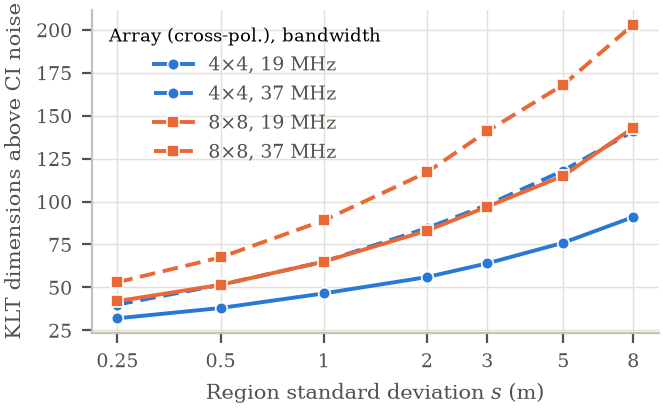
\includegraphics[width=\columnwidth]{fig_dimension}
\caption{Effective dimension of the region twin subspace (KLT dimensions above the CI noise, median over 40 strong links) versus the region standard deviation, for two array sizes and two bandwidths.}
\label{fig:dimension}
\end{figure}

\subsection{Two-Layer Coding}
Energy outside the twin subspace can only be captured by the residual layer. With $N$ angle--delay coefficients of noise variance $\nu$, the threshold $2\nu\ln N$ rejects noise-only coefficients with high probability~\cite{donoho1994ideal}, so the layer stops by itself when the twin is accurate. Lowering the threshold to 0.3 of this value increased the bits by 18--34\% for only 0.1--1.3~bit/s/Hz more sum SE in our setting. \todo{derive the optimal split between the twin and residual layers under the Gaussian model.}

\section{Leakage Law}\label{sec:leakage}

\begin{figure*}[t]
\centering
\begin{minipage}[b]{0.43\textwidth}\centering
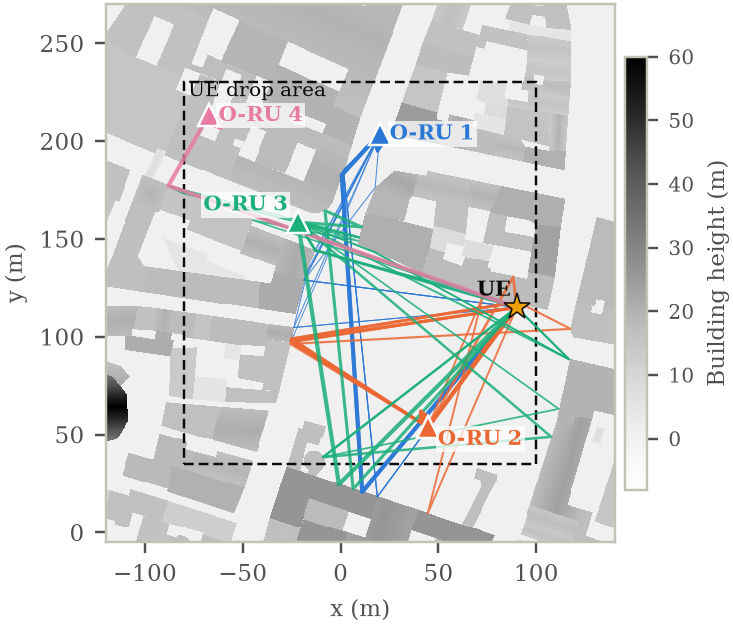
\includegraphics[width=\linewidth]{fig_scene}\\[-1mm]
{\footnotesize (a)}
\end{minipage}\hfill
\begin{minipage}[b]{0.54\textwidth}\centering
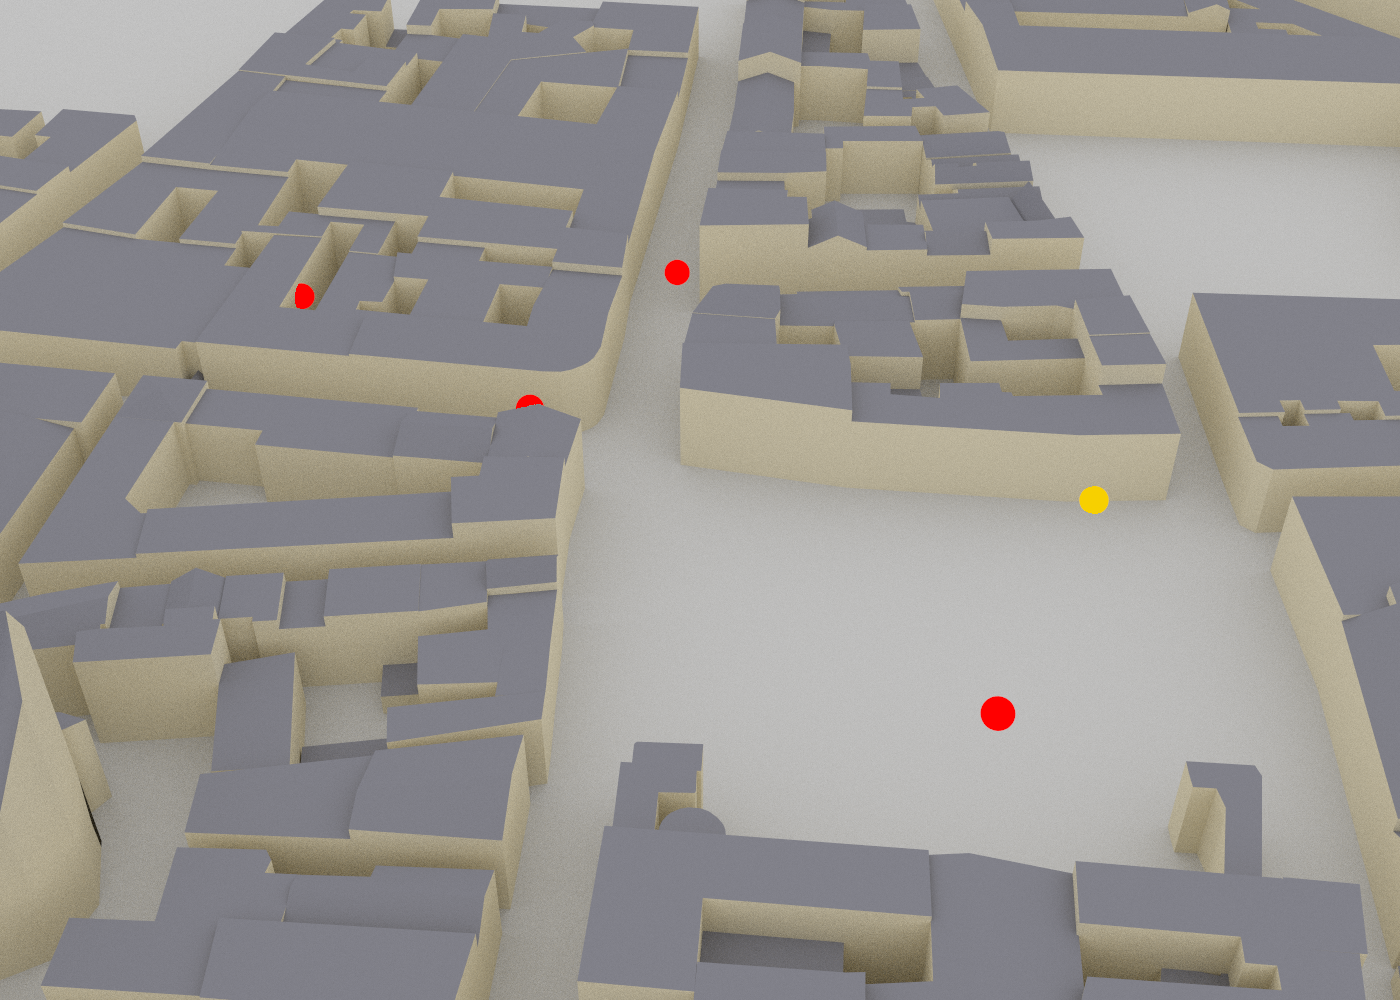
\includegraphics[width=\linewidth]{fig_scene_render}\\[1mm]
{\footnotesize (b)}
\end{minipage}
\caption{The Sionna RT Munich twin used in all experiments. (a) Top view with building heights, the four O-RUs of the $K=8$ runs (arrows: array boresight), the UE drop area, and an example UE with its 12 strongest twin paths to each O-RU (line width by path power over a 30-dB range). The position posterior of this UE for $\sigma=2$~m ($s=2.2$~m) is smaller than the star marker. (b) Perspective view of the same twin from the south; O-RUs in red, the example UE in yellow.}
\label{fig:scene}
\end{figure*}


\subsection{First-Order SINR}
Write the reconstructed channels as $\hat{\vect{h}}_{k}=\vect{h}_{k}+\vect{e}_{k}$ per PRB group. With RZF close to zero forcing, the beam of UE $j\ne k$ is nearly orthogonal to $\hat{\vect{h}}_k$, so UE $k$ receives from it the interference $|\vect{e}_k^{H}\vect{w}_j|^2$. If the error were isotropic with energy $D_k$ over $FN_t$ entries, each of the $K-1$ beams of power $1/K$ would leak $D_k/(KFN_t)$ on average, which gives the term $cD_k$ in~\eqref{eq:proxy}; the signal retains the reconstructed energy $E_k-D_k$ with the zero-forcing gain $a$. The leakage factor
\begin{equation}
\gamma_k=\frac{\sum_{j\ne k}\vect{w}_j^{H}\vect{R}_{\mathrm{err},k}\vect{w}_j}{\frac{K-1}{K}\,\tr(\vect{R}_{\mathrm{err},k})/N_t}
\end{equation}
measures how much more the actual error leaks than an isotropic one, with $\vect{R}_{\mathrm{err},k}$ the error covariance.

\subsection{Why Compression Errors Leak More}
Decomposing the SE loss on exported matrices ($K=8$) shows that the signal loss is below 0.05~dB for the region-twin codes, so the loss is almost entirely interference. White estimation noise leaks 0.89 times the isotropic value, whereas compression errors leak 2--6 times: 13--25\% of a UE's compression error falls into the span of the other UEs' reconstructed channels, against 5.5\% for an isotropic error. In a street canyon, the UEs served by an O-RU share a few dominant directions, and any error in channel-like directions leaks into their beams.

\subsection{Twin Prediction of $\gamma$}
Because $\vect{R}_{\mathrm{err},k}$ and the beams $\vect{w}_j$ can both be approximated from the twin (precoders computed on twin proxy channels, error covariance from the allocated widths and the dropped eigenvalues), $\gamma_k$ can be predicted before any CI is sent. Table~\ref{tab:gamma} shows that $\gamma$ falls with $K$, from about 4 at $K=8$ to about 1 at $K=32$, because more beams spread over more directions, and that the twin predicts it within a factor of two for 96--100\% of the UEs. Two consequences matter in practice. To approach the uncompressed SE, the compression error must be about $\gamma/0.9$ times below the estimation noise, so compression is never free at high SINR; and the bit allocation is insensitive to $\gamma$ (replacing 2.7 by 1 or by per-UE twin predictions changes the sum SE by less than 0.8 percentage points), so $\gamma$ is useful mainly for SE prediction and admission control.

\begin{table}[t]
\centering
\caption{Leakage factor $\gamma$ (median over UEs)}
\label{tab:gamma}
\begin{tabular}{@{}lccc@{}}
\toprule
 & $K=8$ & $K=16$ & $K=32$\\
\midrule
Measured & 4.30 & 3.58 & 1.13\\
Twin prediction (twin proxy precoder) & 3.70 & 3.48 & 1.29\\
Prediction with the actual precoder & 3.89 & 3.48 & 1.28\\
UEs within a factor of 2 (twin) & 100\% & 99\% & 96\%\\
\bottomrule
\end{tabular}
\end{table}

\section{Closed-Loop Position Acquisition}\label{sec:loc}
The region samples double as particles. After reconstructing the CI of UE $k$, the O-DU scores each particle by the energy of $\hat{\vect{h}}_{k}$ captured by that particle's twin path atoms, summed over O-RUs, with a free complex gain per path so that the score ignores the sub-wavelength phase pattern. Tempered importance weights $w_i\propto\exp\{(\mathrm{score}_i-\max\mathrm{score})/(T\|\hat{\vect{h}}_k\|^2)\}$ with $T=10^{-3}$ give the posterior mean $\hat{\vect{x}}_k$ and variance $\sigma_k^2$, to which the particle resolution is added; the next region uses $s_k^2=\sigma_k^2+s_0^2$. The first occasion starts from an external coarse prior and uses 192 particles, later occasions 64. The O-DU localizes on the reconstruction at a budget of 32 coefficients per link, so localization reuses the CI already sent.

\section{Numerical Results}\label{sec:results}

\subsection{Setup}
Table~\ref{tab:setup} lists the parameters. The twin is the Sionna RT~\cite{hoydis2023sionnart} model of a Munich district, with specular reflection and diffraction up to depth 3. The ``reality'' is either the same scene (reality = twin) or a modified one: diffuse scattering with coefficient 0.3 on all surfaces, every building shifted rigidly by $\mathcal{N}(0,0.5^2)$~m per axis, permittivity and conductivity of every material multiplied by log-normal factors with 30\% spread, 40 parked metal cars absent from the twin, or all of these combined. UEs are dropped uniformly in the outdoor area, and the estimated position is the true one plus $\mathcal{N}(\vect{0},\sigma^2\vect{I})$. All schemes see the same drops, CI noise and position errors. Bands are 95\% bootstrap intervals over drops.

Fig.~\ref{fig:scene} shows the site. The four O-RUs of the $K=8$ runs stand on poles in streets and squares of the district and face the center of the $180\times195$~m drop area; the runs with $K=16$ and $K=32$ draw their poles with other seeds under the same rules. The example UE in Fig.~\ref{fig:scene}(a) is 76~m from its nearest O-RU and has 53, 327, 95 and 1 twin paths to O-RUs 1--4. Its channel thus combines a few strong street-canyon reflections with many weak paths, which is the structure the region subspace has to capture.

\begin{table}[t]
\centering
\caption{Simulation parameters}
\label{tab:setup}
\begin{tabular}{@{}ll@{}}
\toprule
Scene & Sionna RT Munich, $180\times195$~m area\\
O-RUs & $L=4$ on 12-m poles, $\ge60$~m apart\\
Array & $4\times4$ cross-pol.\ UPA, $M=32$, 3GPP element\\
Carrier, numerology & 3.5~GHz, 30~kHz, 52 PRBs (18.7~MHz)\\
PRB groups & 2 PRBs, $F=26$, $N=MF=832$\\
UEs & $K\in\{8,16,32\}$, single antenna, 1.5~m\\
Drops & 16 ($K=8$), 8 ($K=16$), 6 ($K=32$)\\
Power & 30~dBm total, UE noise figure 9~dB\\
CI noise & $\nu=1$ (median link NMSE $\approx-29$~dB)\\
Ray tracing & depth 3, $5\times10^5$ rays, diffraction\\
Region & $S=64$, $s_0=1$~m\\
Position error & $\sigma\in\{0,2,5\}$~m\\
Quantizer & noise-matched BFP9, $\kappa=2$\\
Raw CI & $KN\times18$ bit per O-RU (119.8~kbit for $K=8$)\\
\bottomrule
\end{tabular}
\end{table}

\subsection{SE Versus Fronthaul}
Fig.~\ref{fig:main} shows the sum SE versus the fronthaul per O-RU and SRS occasion for $K=8$. When the reality equals the twin, the proposed coder reaches 95\% of the uncompressed sum SE at 1.9~kbit for $\sigma=0$ and at 3.4~kbit for $\sigma=2$~m, 1.6\% and 2.9\% of the raw CI. Its projection also removes estimation noise, so the 5\%-user SE exceeds that of the uncompressed CI by 6--10\% at budgets of 16 coefficients per link and more. Fixed-precision coefficients need 40\% more bits at $\sigma=0$; the point twin, which uses only the paths at $\hat{\vect{x}}$, needs 6.1~kbit and loses most of its advantage at $\sigma=2$~m. The site-wide twin KLT, which ignores the position, reaches 79\% at 11.5~kbit, and the angle--delay DFT, the generic beamspace-type transform, reaches 65\% at about the Gram cost. With diffuse scattering in the reality, the proposed coder reaches 80\% at 5.1~kbit and 90\% at 9.9~kbit; fixed and variable precision then perform alike, because the bits go to the residual layer.

\begin{figure*}[t]
\centering
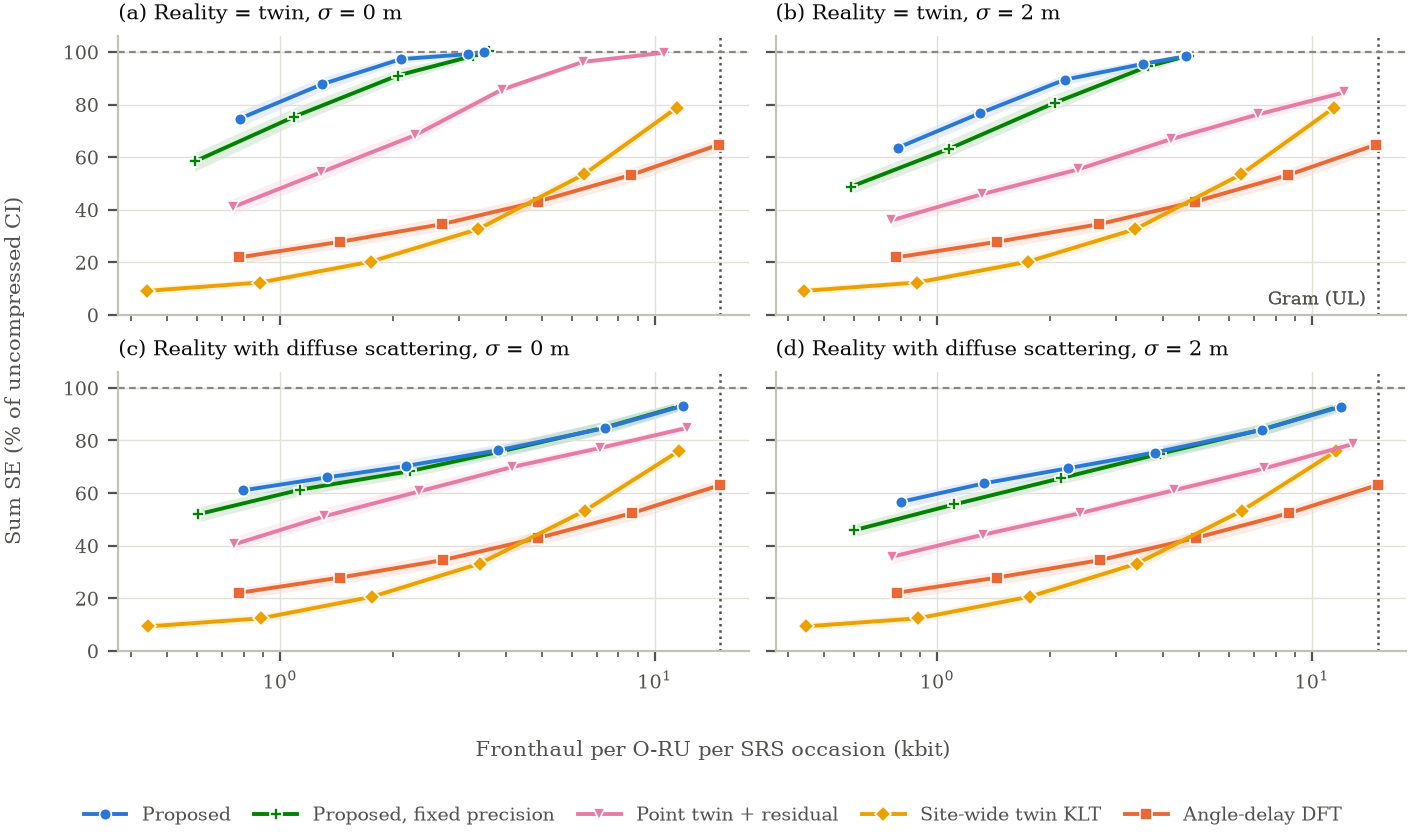
\includegraphics[width=\textwidth]{fig_main_k8}
\caption{Sum SE versus fronthaul per O-RU and SRS occasion, $K=8$, four O-RUs. The dotted vertical line is the uplink cost of exact distributed Gram RZF.}
\label{fig:main}
\end{figure*}

\subsection{Scaling With the Number of UEs}
Table~\ref{tab:bits} and Fig.~\ref{fig:kscale} compare the bits needed for a target fraction with the Gram uplink cost. The proposed coder grows roughly linearly with $K$, Gram RZF quadratically. When the reality equals the twin, 95\% costs 1.9, 4.9 and 7.7~kbit for $K=8,16,32$, i.e., 12.5\%, 8.2\% and 3.2\% of the Gram uplink cost alone; at $\sigma=2$~m the numbers are 3.4, 9.7 and 14.2~kbit. With diffuse scattering, 90\% costs 9.9, 26.9 and 59.4~kbit (66\%, 45\% and 25\% of Gram uplink), and at $K=32$ the proposed coder saturates at 90\%, whereas Gram RZF is exact. Combinatorial index coding is what makes 90\% reachable here: with per-index coding the same residual layer saturated at 85--88\%.

\begin{table}[t]
\centering
\caption{kbit per O-RU and SRS occasion to reach a fraction of the uncompressed sum SE}
\label{tab:bits}
\begin{tabular}{@{}lrrrr@{}}
\toprule
 & Proposed & Fixed prec. & Grid cell & Gram UL\\
\midrule
\multicolumn{5}{@{}l}{\emph{Reality = twin, 95\%}}\\
$K=8$, $\sigma=0$ & 1.87 & 2.64 & 2.67 & 15.0\\
$K=8$, $\sigma=2$~m & 3.42 & 3.76 & 4.16 & 15.0\\
$K=8$, $\sigma=5$~m & 7.22 & 7.14 & n.r.\ (92.6\%) & 15.0\\
$K=16$, $\sigma=0$ & 4.9 & 6.9 & 7.2 & 59.9\\
$K=16$, $\sigma=2$~m & 9.7 & 10.6 & 12.1 & 59.9\\
$K=32$, $\sigma=0$ & 7.7 & 10.0 & 10.2 & 239.6\\
$K=32$, $\sigma=2$~m & 14.2 & 16.4 & 23.4 & 239.6\\
\midrule
\multicolumn{5}{@{}l}{\emph{Reality with diffuse scattering, 90\%}}\\
$K=8$, $\sigma=0$ & 9.9 & 9.8 & 10.1 & 15.0\\
$K=16$, $\sigma=0$ & 26.9 & 26.5 & 27.1 & 59.9\\
$K=32$, $\sigma=0$ & 59.4 & 58.9 & n.r.\ (89.8\%) & 239.6\\
\bottomrule
\multicolumn{5}{@{}l}{\footnotesize n.r.: not reached within 128 coefficients per link (best fraction).}
\end{tabular}
\end{table}

\begin{figure*}[t]
\centering
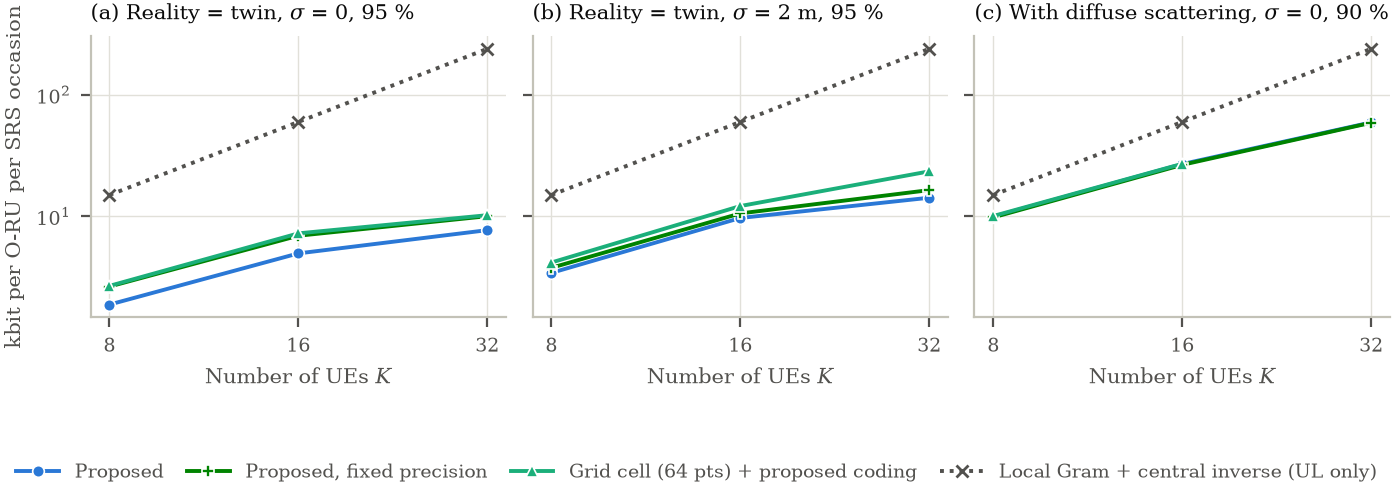
\includegraphics[width=\textwidth]{fig_kscale}
\caption{Fronthaul per O-RU and SRS occasion needed for a target fraction of the uncompressed sum SE versus the number of UEs, compared with the uplink cost of exact distributed Gram RZF.}
\label{fig:kscale}
\end{figure*}

\subsection{What the Position and the Twin Contribute}
Fig.~\ref{fig:ablation} isolates the role of the prior. Replacing the posterior region by the $5\times5$~m grid cell that contains $\hat{\vect{x}}$ (64 twin points, all other parts of the coder unchanged) costs 32--47\% more bits at $\sigma=0$ and 22--65\% more at $\sigma=2$~m across $K$, and at $\sigma=5$~m the grid version no longer reaches 95\% (Table~\ref{tab:bits}). Building the grid basis from the four cell vertices only, as in~\cite{cai2025ecb}, limits each link to four dimensions in a static scene; with our allocation and residual layer this reaches 77\%, and as a plain truncation 36\%. Data-driven codes trained on the twin over the whole site do not use the position and saturate: the site-wide KLT reaches 79\% at about 12~kbit and a twin-trained autoencoder~\cite{wen2018csinet,luo2025dtfeedback} with the estimated position as input about 40\%.

Fig.~\ref{fig:aestudy} explains the saturation. On held-out twin channels, autoencoders with nested dropout~\cite{rippel2014nested} beat the linear site-wide KLT at small latent sizes (about $-9$~dB against $-4$~dB at 16 dimensions) but plateau at about $-10$~dB; one model per latent size, or a learned correction on top of the KLT, reaches $-12$ to $-13.5$~dB at 128 dimensions, no better than the KLT itself. Longer training did not help and once diverged. Centralized RZF needs the compression error to stay below the estimation noise (median link NMSE about $-29$~dB here, Section~\ref{sec:leakage}), which a position-agnostic code does not approach within these budgets.

\begin{figure*}[t]
\centering
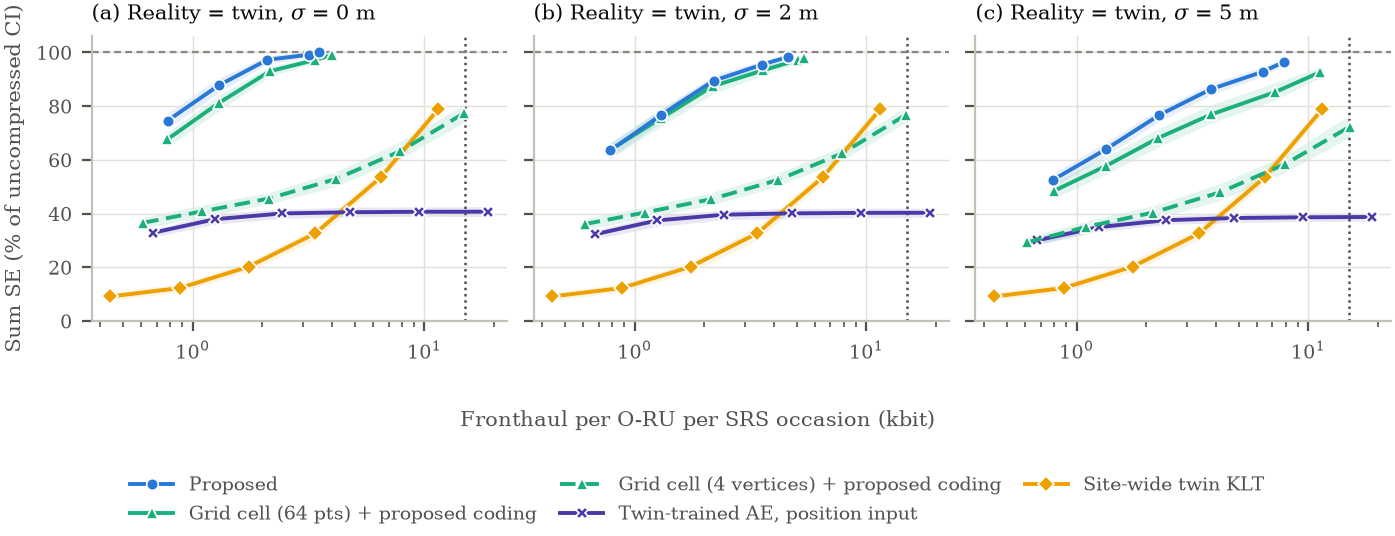
\includegraphics[width=\textwidth]{fig_ablation}
\caption{Role of the prior, $K=8$, reality = twin: posterior region (proposed) versus the grid cell around $\hat{\vect{x}}$ with 64 points or its four vertices (same coder), a twin-trained autoencoder with position input, and a site-wide twin KLT.}
\label{fig:ablation}
\end{figure*}

\begin{figure}[t]
\centering
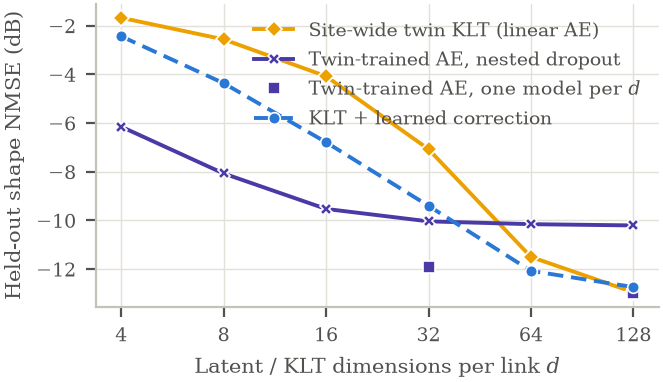
\includegraphics[width=\columnwidth]{fig_ae_study}
\caption{Held-out NMSE of the normalized channel shape of twin-trained codes versus the latent size per link (O-RUs 1 and 2, 20\,556 training and 2\,284 test positions, CI noise included).}
\label{fig:aestudy}
\end{figure}

\subsection{Twin Mismatch}
Fig.~\ref{fig:mismatch} reports the sum SE relative to the uncompressed CI in the same reality. At 128 coefficients per link (about 4--15~kbit), the proposed coder retains 99\% without mismatch, 95\% with buildings shifted by 0.5~m, 93\% with 40 unmodeled cars, 91\% with unmodeled diffuse scattering, 90\% with $\pm30\%$ material errors and 75\% with all of them combined, against 53--58\% for the angle--delay DFT. At 32 coefficients per link the losses are larger (97, 87, 77, 74, 71 and 57\%) because the residual layer has fewer bits. The material case is severe because the twin models walls as 10-cm dielectric slabs, whose reflection coefficient is very sensitive to the permittivity (median relative error 112\% for $\pm30\%$, against 0.8\% for a half-space). Under mismatch the grid prior and fixed precision come within two percentage points of the proposed coder: the twin error, not the region shape, then dominates.

\begin{figure*}[t]
\centering
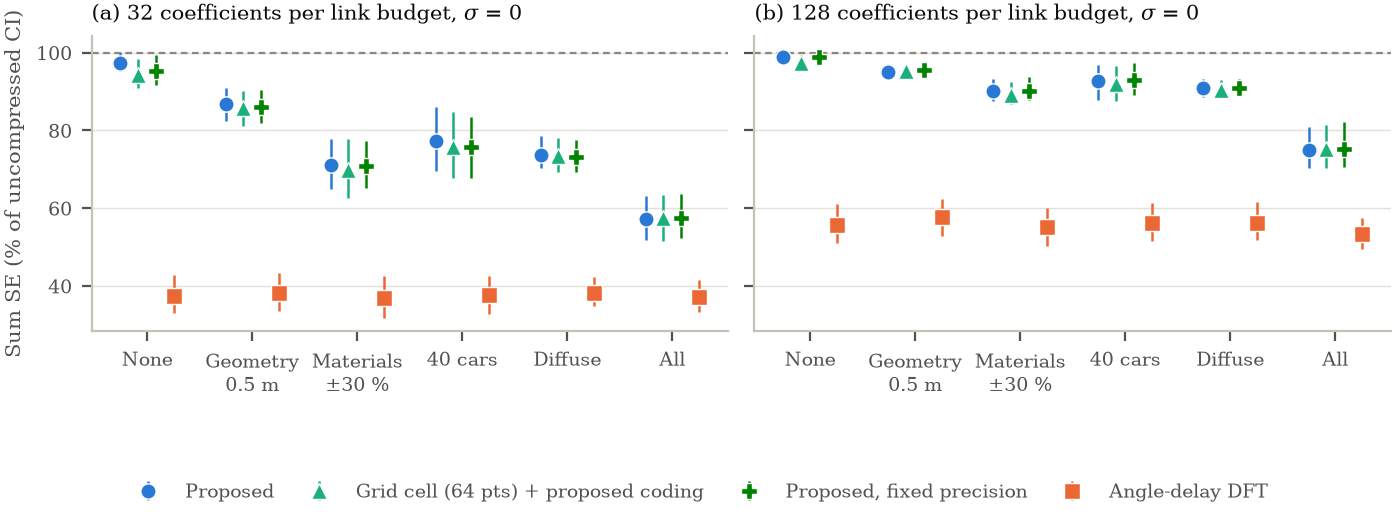
\includegraphics[width=\textwidth]{fig_mismatch}
\caption{Sum SE under twin mismatch, $K=8$, six drops, $\sigma=0$, as a fraction of the uncompressed CI in the same reality.}
\label{fig:mismatch}
\end{figure*}

\subsection{Closed-Loop Localization}
Fig.~\ref{fig:tracking} starts from an external prior with 5 or 10~m error. After three SRS occasions the median localization error is 0.20--0.28~m when the reality equals the twin and 0.38--0.39~m with diffuse scattering, and the sum SE at 32 coefficients per link is at least 98\% of the SE with known positions. About 10\% of the UEs remain at a wrong location (90th percentile 2.0--3.5~m, or 10~m from a 10-m prior with diffuse scattering) with little effect on the sum SE.

\begin{figure*}[t]
\centering
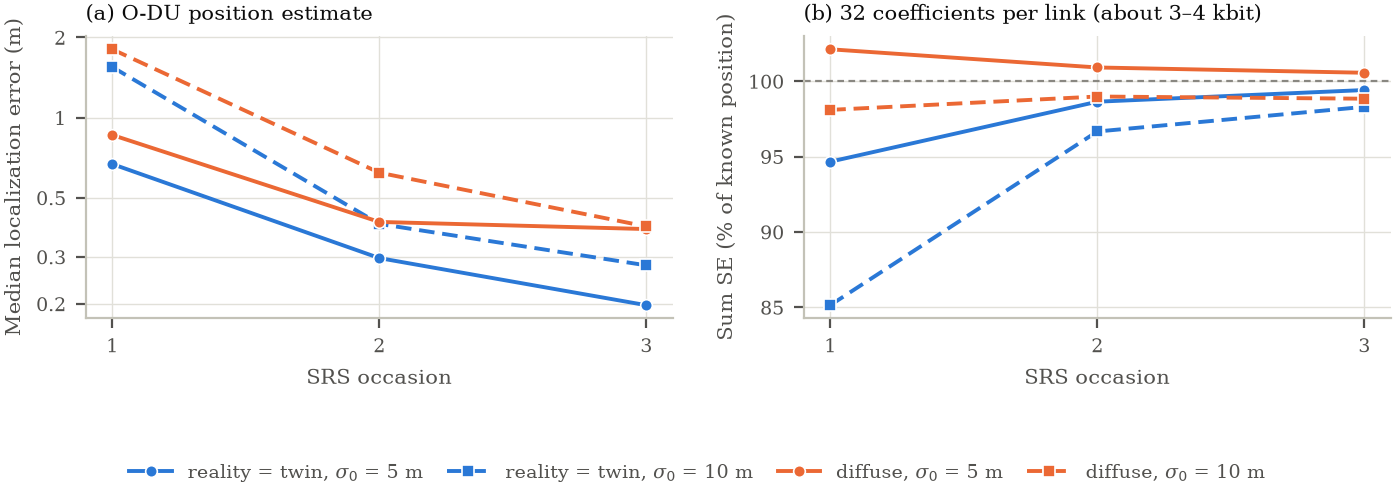
\includegraphics[width=\textwidth]{fig_tracking}
\caption{Closed-loop O-DU localization with the proposed coder, $K=8$: (a) median localization error, (b) sum SE relative to known positions.}
\label{fig:tracking}
\end{figure*}

\subsection{Per-O-RU Power Constraint}
Scaling the RZF precoder so that no O-RU exceeds $1/L$ of the total power changes the bits for 95\% from 1.87, 3.42 and 7.22~kbit to 1.83, 3.26 and 6.97~kbit ($\sigma=0,2,5$~m, reality = twin) and keeps the ranking of all schemes.

\section{Discussion}
\emph{Where the twin stops helping.} Diffuse scattering and material errors are components the twin cannot represent, and only the residual layer can pay for them. In that regime the coder still uses a small fraction of the Gram cost up to 80--90\% of the uncompressed SE, but exact Gram RZF is the better choice above that. Modeling diffuse scattering in the twin recovers only 6--7 percentage points, because diffuse fields are made of many weak paths whose phases change on the wavelength scale and are not captured by 64 region samples.

\emph{Limitations.} The ``reality'' is a perturbed ray-tracing model of one district, not a measurement; UEs are static within a drop; SE is the Shannon rate of RZF rather than link-level throughput. Using the scheme in O-RAN requires a new CI compression method in the SRS CI conveyance and a mechanism that keeps the twin version and the posterior synchronized between the O-DU and the O-RUs.

\section{Conclusion}
A digital twin shared by the O-DU and the O-RUs turns fronthaul compression of SRS channel information into source coding with a common prior. Building the code over the position posterior, allocating bits by twin eigenvalues for the centralized precoder, and adding a residual layer for what the twin misses reduces the CI needed for 95\% of the uncompressed sum SE to a few kbit per O-RU and SRS occasion, far below exact distributed Gram precoding, with a gap that widens as the number of UEs grows. The redundancy of the code decomposes into basis and allocation mismatch, and its SE cost follows a leakage law that the twin predicts. Future work concerns online twin calibration from the decoded CI, its synchronization between O-DU and O-RUs, and the downlink counterpart for CSI-RS port design.

\appendices
\section{Proof of Proposition~\ref{prop:redundancy}}\label{app:proof}
With rates $r_i=\log_2(\hat c_i/\hat\theta)$ the distortion is $\hat D=\sum_ic_i2^{-r_i}=\hat\theta\sum_i\rho_i$ and the rate is $\hat R=\sum_i\log_2(\hat c_i/\hat\theta)$. The KLT of $\vect{C}$ with optimal rates reaches the same distortion $\hat D$ with equal per-coefficient distortion $\hat D/N$ and rate $R^\star=\sum_i\log_2(\mu_i N/\hat D)$. Hence
\begin{align*}
\hat R-R^\star&=\sum_i\log_2\hat c_i-\sum_i\log_2\mu_i+N\log_2\frac{\hat D}{N\hat\theta}\\
&=\Big[\sum_i\log_2c_i-\log_2\det\vect{C}\Big]\\
&\quad+N\log_2\mathrm{AM}(\rho)-\sum_i\log_2\rho_i,
\end{align*}
using $\sum_i\log_2\mu_i=\log_2\det\vect{C}$ and $\sum_i\log_2\hat c_i=\sum_i\log_2c_i-\sum_i\log_2\rho_i$. Since $\sum_i\log_2\rho_i=N\log_2\mathrm{GM}(\rho)$, this is~\eqref{eq:redundancy}. Hadamard's inequality gives $\prod_ic_i\ge\det\vect{C}$ and the AM--GM inequality the nonnegativity of the second term. For the bound,
\begin{align*}
D_{\mathrm{KL}}&=\tr(\hat{\vect{C}}^{-1}\vect{C})-\ln\det(\hat{\vect{C}}^{-1}\vect{C})-N\\
&=N\big[\mathrm{AM}(\rho)-1-\ln\mathrm{GM}(\rho)\big]\\
&\quad+\Big[\sum_i\ln c_i-\ln\det\vect{C}\Big],
\end{align*}
and $\mathrm{AM}-1\ge\ln\mathrm{AM}$ gives $\Delta R\,\ln2\le D_{\mathrm{KL}}$.

\bibliographystyle{IEEEtran}
\bibliography{refs}

\end{document}
